\documentclass{beamer}
\mode<presentation>
\usepackage{amsmath}
\usepackage{amssymb}
%\usepackage{advdate}
\usepackage{graphicx}
\graphicspath{{./figs/}}
\usepackage{adjustbox}
\usepackage{subcaption}
\usepackage{enumitem}
\usepackage{multicol}
\usepackage{mathtools}
\usepackage{listings}
\usepackage{url}
\def\UrlBreaks{\do\/\do-}
\usetheme{Boadilla}
\usecolortheme{lily}
\setbeamertemplate{footline}
{
  \leavevmode%
  \hbox{%
  \begin{beamercolorbox}[wd=\paperwidth,ht=2.25ex,dp=1ex,right]{author in head/foot}%
    \insertframenumber{} / \inserttotalframenumber\hspace*{2ex} 
  \end{beamercolorbox}}%
  \vskip0pt%
}
\setbeamertemplate{navigation symbols}{}

\providecommand{\nCr}[2]{\,^{#1}C_{#2}} % nCr
\providecommand{\nPr}[2]{\,^{#1}P_{#2}} % nPr
\providecommand{\mbf}{\mathbf}
\providecommand{\pr}[1]{\ensuremath{\Pr\left(#1\right)}}
\providecommand{\qfunc}[1]{\ensuremath{Q\left(#1\right)}}
\providecommand{\sbrak}[1]{\ensuremath{{}\left[#1\right]}}
\providecommand{\lsbrak}[1]{\ensuremath{{}\left[#1\right.}}
\providecommand{\rsbrak}[1]{\ensuremath{{}\left.#1\right]}}
\providecommand{\brak}[1]{\ensuremath{\left(#1\right)}}
\providecommand{\lbrak}[1]{\ensuremath{\left(#1\right.}}
\providecommand{\rbrak}[1]{\ensuremath{\left.#1\right)}}
\providecommand{\cbrak}[1]{\ensuremath{\left\{#1\right\}}}
\providecommand{\lcbrak}[1]{\ensuremath{\left\{#1\right.}}
\providecommand{\rcbrak}[1]{\ensuremath{\left.#1\right\}}}
\theoremstyle{remark}
\newtheorem{rem}{Remark}
\newcommand{\sgn}{\mathop{\mathrm{sgn}}}
\providecommand{\abs}[1]{\left\vert#1\right\vert}
\providecommand{\res}[1]{\Res\displaylimits_{#1}} 
\providecommand{\norm}[1]{\lVert#1\rVert}
\providecommand{\mtx}[1]{\mathbf{#1}}
\providecommand{\mean}[1]{E\left[ #1 \right]}
\providecommand{\fourier}{\overset{\mathcal{F}}{ \rightleftharpoons}}
%\providecommand{\hilbert}{\overset{\mathcal{H}}{ \rightleftharpoons}}
\providecommand{\system}[1]{\overset{\mathcal{#1}}{ \longleftrightarrow}}
%\providecommand{\system}{\overset{\mathcal{H}}{ \longleftrightarrow}}
	%\newcommand{\solution}[2]{\textbf{Solution:}{#1}}
%\newcommand{\solution}{\noindent \textbf{Solution: }}
\providecommand{\dec}[2]{\ensuremath{\overset{#1}{\underset{#2}{\gtrless}}}}
\newcommand{\myvec}[1]{\ensuremath{\begin{pmatrix}#1\end{pmatrix}}}
\let\vec\mathbf

\lstset{
%language=C,
frame=single, 
breaklines=true,
columns=fullflexible
}

\numberwithin{equation}{section}

\title{1.6.16}
\author{AI25BTECH11001 - ABHISEK MOHAPATRA}
\begin{document}
\maketitle
% \newpage
% \bigskip

		\textbf{Question}:

		\noindent Find the values of $k$ if the points $\vec{A}(k +1,2k)$, $\vec{B}(3k, 2k +3)$ and $\vec{C}(5k-1,5k)$ are collinear.

		\textbf{Solution:} From the given information,


		\begin{align}
			\vec{A} = \myvec{k+1\\2k},\vec{B} = \myvec{3k\\2k+3},\vec{C} = \myvec{5k-1\\5k} 
		\end{align}
		To check if the points are collinear, we can use 
		\begin{align}
			rank\myvec{\vec{B}-\vec{A} & \vec{C}-\vec{A}} = 1	
		\end{align}
		So,
		\begin{align}
			\myvec{\vec{B}-\vec{A} & \vec{C}-\vec{A}}^T = \myvec{2k-1 & 3 \\ 4k-2 & 3k}	
			\\
			\xleftrightarrow[]{R_2 = R_2 - 2R_1} 
			\myvec{2k-1 & 3 \\ 0 & 3k-6} 
		\end{align}
		The rank of the matrix will be 1 when 
		\begin{align}
		3k-6 = 0
		\end{align}
		\begin{align}
		\Rightarrow k = 2
		\end{align}
		Graph:
\begin{figure}[H]
	\centering
	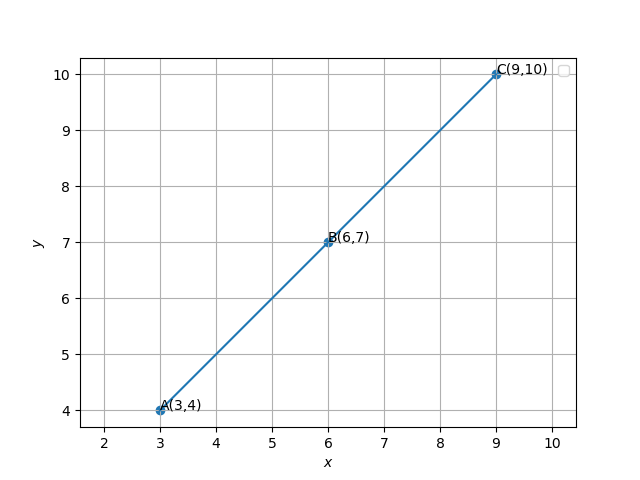
\includegraphics[scale=0.5]{img}
	\caption*{}
	\label{img}
\end{figure}


		Therefore, k = 2.
\end{document}

